\documentclass[a4paper, 8pt]{extarticle}

\usepackage[greek,spanish,es-tabla,es-nodecimaldot,es-noindentfirst]{babel}

\usepackage[a4paper, lmargin=0.2cm,rmargin=0.2cm,tmargin=0.2cm,bmargin=0.2cm, landscape]{geometry}
\usepackage{multicol}
\usepackage{amsmath}
\usepackage{mathtools}
\usepackage{cancel}
\usepackage{siunitx}
\usepackage{physics}
\usepackage{enumitem}
\usepackage{circuitikz}
\usepackage{graphicx}
\usepackage{xcolor}
\usepackage{xspace}

% For Excel2LaTeX tables
\usepackage{colortbl}
\usepackage{booktabs}

\AtBeginDocument{\RenewCommandCopy\qty\SI}
\usepackage{esvect}
\renewcommand{\vec}[1]{\vv{{#1}}}
\renewcommand{\grad}{\nabla}

\usepackage{lmodern}
\renewcommand{\familydefault}{\sfdefault}
\renewcommand{\rmdefault}{\sfdefault}

\renewcommand{\sin}{\sen}

\usepackage{titlesec}
\titleformat{\section}
  {\normalfont\Large\bfseries}{\thesection}{1em}{}[{\titlerule[0.8pt]}]

\titlespacing*{\section}{0pt}{4pt plus 0pt minus 0pt}{5pt plus 2pt minus 2pt}
\titlespacing*{\subsection}{0pt}{4pt plus 0pt minus 0pt}{3pt plus 2pt minus 2pt}
\titlespacing*{\subsubsection}{0pt}{4pt plus 0pt minus 0pt}{3pt plus 2pt minus 2pt}

\allowdisplaybreaks
\setcounter{secnumdepth}{-1}
\setcounter{tocdepth}{-1}

%%% INICIO DEL DOCUMENTO %%%
\begin{document}

\setlength{\parskip}{0pt}
\setlength{\parindent}{0pt}
\setlist{nosep}
\setlength{\abovedisplayskip}{2pt}
\setlength{\belowdisplayskip}{2pt}
\setlength{\abovedisplayshortskip}{0pt}
\setlength{\belowdisplayshortskip}{0pt}


\pagestyle{empty}
\renewcommand{\arraystretch}{1.5}

\begin{multicols}{3}
  \section{T3. Micrófonos}
  \subsection{Características de los micrófonos}
  \subsubsection{Sensibilidad}
  La sensibilidad de un micrófono es la \textbf{relación entre la tensión eléctrica generada y la presión acústica incidente} (en circuito abierto, campo libre, a \qty{1}{\kilo\hertz}).
  \begin{align*}
    S & = \frac{E_{\text{c.a.}}}{p} \ \left[ \unit{\volt \per \pascal }  \right]                                                                            \\
      & = 20 \log \left( \frac{\abs{S}}{\qty{1}{\volt \per \pascal  } } \right) \ \left[ \unit{\decibel} \text{ re. } \qty{1}{\volt \per \pascal }  \right]
  \end{align*}
  La sensibilidad de referencia es la sensibilidad medida en el eje del micrófono.
  \[ S_0 = S \left( \theta = \ang{0} \right) \]
  \subsubsection{Respuesta en frecuencia}
  La respuesta en frecuencia de un micrófono es la \textbf{variación de la sensibilidad con la frecuencia} $\left[ S = S(f) \right]$. Se suele representar la respuesta relativa con respecto a la sensibilidad de referencia en decibelios.
  \[ S(f) - S_0 = 20 \log \left( \frac{\abs{S(f)}}{\abs{S_0}} \right) \ \unit{\dB} \]
  La presencia del micrófono afecta a su respuesta. La respuesta del diafragma en alta frecuencia aumenta la presión frente a la cápsula.

  \color{red}\xspace
  \subsubsection{Distorsión lineal}
  \begin{itemize}
    \item \textbf{Coloraciones.} La respuesta en frecuencia no es plana.
    \item \textbf{Vibraciones parciales del diafragma.} Debidas a modos propios. Los micros de condensador no tienen este problema.
    \item \textbf{Resonancias mecánicas o acústicas.} Sobre todo en micros dinámicos.
    \item \textbf{Ancho de banda limitado por componentes eléctricos.}
    \item \textbf{Distorsión de fase.}
  \end{itemize}
  \subsubsection{Distorsión no lineal}
  \begin{itemize}
    \item \textbf{Saturación.} Sobrecarga de presión. Si saturan fácilmente se llaman micros \textit{blandos}. Si no, \textit{duros}.
    \item \textbf{Pop.} Chorros de aire (no sonido). Suele ser por fonemas ``explosivos''.
  \end{itemize}
  \color{black}\xspace
  \subsubsection{Directividad}
  Generalmente, su supone simetría cilíndrica de los micrófonos, por lo que la directividad no depende del plano azimutal $\varphi$.
  \begin{align*}
    D(\theta, \varphi )          & \equiv \text{Directividad}                                         \\
    Q(\theta, \varphi )          & \equiv \text{Factor de directividad}                               \\
    Q _{\textnormal{ax}}         & \equiv \text{Factor de directividad axial (en el eje)}             \\
    \text{DI}                    & \equiv \text{Índice de directividad}                               \\
    \text{DI} _{\textnormal{ax}} & \equiv \text{Índice de directividad axial (en el eje)}             \\
    \text{REE}                   & \equiv \text{Eficiencia de energía aleatoria}                      \\
    \text{DSF}                   & \equiv \text{Factor de distancia}                                  \\
    E_d                          & \equiv \text{Tensión directa}                                      \\
    E_r                          & \equiv \text{Tensión reverberante}                                 \\
    E_{ro}                       & \equiv \text{Tensión reverberante del equivalente omnidireccional} \\
  \end{align*}

  Si especifican que se ha medido en cámara anecoica, entonces se refiere a que $E_{\text{c.a.}}$ es también el valor de $E_d$.
  \begin{align*}
    p_d (r) & = \frac{p (\qty{1}{\metre } )}{r} \qquad E_d = p_d (r) S                                                                  \\
    E_r     & = \frac{p_r S_0}{\sqrt{Q _{\textnormal{ax}}}} \qquad \langle E_d^2(\theta, \varphi) \rangle = E_r^2 \qquad E_{ro} = p_r S
  \end{align*}
  La distancia crítica $r_c$ es la distancia a partir de la cual la presión reverberante es igual a la directa. En ella la tensión total y presión total serán:
  \begin{align*}
    E_{t}           & = \sqrt{E_r ^2 + E_d ^2}                   & p_0 = p_r = p_d = \frac{p_{t}}{\sqrt{2}} \\
    E_{t} (\theta ) & = p_0 S_0 \sqrt{D^2(\theta ) + \text{REE}}
  \end{align*}
  Recordamos que es suma no coherente por ser campo difuso.
  \begin{align*}
    D( \theta)          & = \frac{S(\theta)}{S_0 } \qquad Q(\theta, \varphi ) = Q _{\textnormal{ax}} D^2                                                    (\theta, \varphi )                                                                              \\
    Q(\theta, \varphi ) & = \frac{S^2(\theta, \varphi )}{\langle S^2(\theta, \varphi) \rangle} = \frac{S^2(\theta, \varphi )}{\frac{1}{4\pi} \int_{\varphi = 0}^{2\pi} \int_{\theta = 0}^{\pi} S^2(\theta, \varphi) \sin (\theta ) \dd \theta \dd \varphi } \\
    Q_{\textnormal{ax}} & = Q(\theta = \ang{0}) = \frac{2}{\int_{\theta = 0}^{\pi} D^2(\theta) \sin (\theta ) \dd \theta } \approx \frac{2}{\frac{\pi}{N} \sum _{i=1}^{N} D^2(\theta _i) \sin (\theta _i)}                                                  \\
    Q_{\textnormal{ax}} & = \frac{E^2_{ro}} {E^2_r} \eval*{}_{\text{campo difuso}} \quad \text{DI} = 10 \log \left[ Q( \theta, \varphi) \right] \qquad \text{DI} _{\textnormal{ax}} = 10 \log \left( Q_{\textnormal{ax}} \right)                            \\
    \text{REE}          & = \frac{1}{Q_ {\textnormal{ax}}} \qquad \text{DSF} = \sqrt{Q_{\textnormal{ax}}}                                                                                                                                                   \\
  \end{align*}

  \textbf{Nota 1:} En la fórmula de $Q_{\textnormal{ax}}$ para $N$ valores, si nos dicen que supongamos simetría de revolución se usan los valores entre $\theta = \ang{0}$ y $\theta = \ang{180}$, sin incluir este último. Si da tiempo (y en entornos reales), se calculan tanto en el intervalo $[0, 180)$ como en $[180, 360)$ y se hace la media entre ambos $Q_{\textnormal{ax}}$ obtenidos.

  \textbf{Nota 2:} Si nos piden sacar la directividad sabiendo que es de familia cardioide y no dicen nada más, debemos suponer orden $n=1$.
  \subsubsection{Directividad de la familia cardiode}
  $A$ es el componente omnidireccional, $B$ el componente bidireccional y $n$ el orden de la directividad.

  \[\left\lbrace
    \begin{matrix*}[l]
      D (\theta ) = \left[ A + B \cos (\theta ) \right] \cos ^{n-1} (\theta )  \\
      A + B = 1
    \end{matrix*}\right.\]


  % Table generated by Excel2LaTeX from sheet 'Sheet1'
  \begin{center}
    \begin{tabular}{|c|c|l|}
      \hline
      \rowcolor[rgb]{ .663,  .816,  .557} A    & B    & \multicolumn{1}{c|}{Tipo} \\
      \hline
      \rowcolor[rgb]{ .886,  .937,  .855} 0.50 & 0.50 & Cardioide                 \\
      \hline
      \rowcolor[rgb]{ .886,  .937,  .855} 0.75 & 0.25 & Subcardioide              \\
      \hline
      \rowcolor[rgb]{ .886,  .937,  .855} 0.25 & 0.75 & Hipercardioide            \\
      \hline
    \end{tabular}
  \end{center}

  Si $n = 1$, el valor de $Q _{\textnormal{ax}}$ viene dado por la resolución de la integral de su definición, el resultado es este:

  \[ Q _{\textnormal{ax}} = \frac{3}{4B^2 - 6B + 3} \]

  \color{red}\xspace
  \subsubsection{Ruido eléctrico}

  \begin{itemize}
    \item \textbf{Ruido eléctrico.} Tensión de salida del micrófono cuando no recibe excitación acústica. Causado por:
          \begin{itemize}
            \item Agitación térmica de moléculas de aire o del diafragma.
            \item Agitación térmica electrónica, debi principalmente a resistencias altas.
          \end{itemize}
          \[ E_N = \sqrt{4kTR \Delta f} \ \left[ \unit{\volt }  \right]\]
          Donde $k$ es la constante de Boltzmann, $T$ la temperatura, $R$ la resistencia y $\Delta f$ el ancho de banda. Se suele expresar en \unit{\dB_{\text{SPL}}} y se denomina ``nivel de presión sonora equivalente al ruido'':
          \[ \text{ENL} = 20 \log \left( \frac{p_N}{p _{\textnormal{ref}}} \right)  = 20 \log \left( \frac{E_N}{p _{\textnormal{ref}}S_0} \right) \]
          Donde $p _{\textnormal{ref}} = \qty{20}{\micro\pascal }$. Para usar esta expresión, mencionar que se debería filtrar $E_N$ con un filtro de ponderación A.
    \item \textbf{Ruido por zumbido electromagnético (\textit{hum}).}
    \item \textbf{Ruido por viento.}
  \end{itemize}

  \subsubsection{Márgenes dinámicos}

  \begin{align*}
    \text{Margen dinámico}        & \qquad \text{DR} = \text{SPL}_{\text{máx}} - \text{ENL}                                    \\
    \text{Margen de sobrecarga}   & \qquad \text{HR} = \text{SPL}_{\text{máx}} - 94 \ (\text{viene de } p _{\textnormal{ref}}) \\
    \text{Relación señal a ruido} & \qquad \text{SNR} = \text{DR} - \text{HR} = 94 - \text{ENL}
  \end{align*}
  \color{black}\xspace
  \subsection{Tipos de micrófonos}
  \subsubsection{TAM: Micrófonos de presión}
  La cápsula está compuesta por un diafragma y un pequeño orificio de ecualización, que sirve para regular la presión interna. La vibración del diafragma es proporcional a la presión acústica externa ejercida sobre el diafragma.
  \begin{center}
    \includegraphics[width=0.8\linewidth]{Mic de presión.png}
  \end{center}
  Presentan un comportamiento omnidireccional, excepto a alta frecuencia debido a difracción cuando $\lambda >> D$, siendo $D$ la mayor dimensión del micrófono. Para $\theta = \pm \ang{90}$, la directividad disminuye ligeramente por falta de uniformidad. Para $\theta = \ang{180}$, la directividad disminuye ligeramente por la sombra que genera la cápsula.

  \subsubsection{TAM: Micrófonos de gradiente de presión}

  La presión en la cara interna del diafragma es aproximadamente igual que en la cara externa. La diferencia de caminos acústicos entre ambas caras es la que hace que no sean iguales. Por lo tanto existe un incremento muy pequeño de presión entre ambas caras, es decir, un diferencial. De ahí viene el término gradiente de presión.
  \vspace*{\fill}
  \begin{center}
    \includegraphics[width=0.4\linewidth]{Mic grad de presión.png}
  \end{center}

  El \textbf{efecto proximidad} sucede cuando $kx << 1$ e implica que para bajas frecuencias (o micro muy cerca de la fuente) las ondas presentan divergencia esférica. Es decir, acercar el micro a la fuente incrementará la tensión generada. Esto no sucede para agudos porque $kx >> 1$ y las ondas son planas (sin divergencia esférica).
  \includegraphics[width=\linewidth]{Gradiente de presión.png}

  \[ \left\lbrace
    \begin{matrix*}[l]
      \lambda >> \Delta L & \longrightarrow D (\theta ) = \cos (\theta )\\
      \lambda << \Delta L & \longrightarrow \abs{D (\theta )} = \abs{\sin \left( \frac{k \Delta L \cos (\theta)}{2} \right)}
    \end{matrix*} \right. \]

  Como el efecto proximidad sucede si $kx << 1$, entonces $f _{\textnormal{prox}} = \frac{c}{2 \pi x}$. Teniendo que $F$ es la fuerza ejercida sobre el diafragma, entonces:

  \begin{align*}
    F                      & = 2jp e^{- \frac{jk \Delta L \cos (\theta)}{2}} \sin \left( \frac{k \Delta L \cos (\theta)}{2} \right) S_d \\
    G _{\textnormal{prox}} & = \frac{F}{F _{\textnormal{ondas planas}}} = \frac{1 + jkx}{jkx}
  \end{align*}

  \subsubsection{TAM: Micrófonos combinados de presión/gradiente de presión}
  Son como los micrófonos de presión cambiando el orificio de ecualización por una abertura de mayor tamaño, conformando un sistema acústico. El principio de funcionamiento es el mismo que los micrófonos de gradiente de presión.
  \begin{align*}
     & \left( k \dd L << 1 \right) \equiv \left( \dd L << \lambda \right)                                                             \\
     & \left\lbrace
    \begin{matrix*}[l]
      k \dd L << 1 & \longrightarrow D (\theta ) = \frac{K + \cos (\theta)}{K + 1}                                                      \\
      k \dd L >> 1 & \longrightarrow \abs{D (\theta )} = \abs{\sin \left( \frac{k\Delta L \left[ \cos (\theta + K) \right]}{2} \right)}
    \end{matrix*} \right. \\
     & \left\lbrace
    \begin{matrix*}[l]
      K = 1 \ \rightarrow \text{ cardioide} \\
      K = \frac{1}{3} \ \rightarrow \text{ hipercardioide} \\
      K = 0 \ \rightarrow \text{ bidireccional} \\
      K > 1 \ \rightarrow \text{ subcardioide}
    \end{matrix*}
    \right.  \qquad  A = \frac{K}{K + 1} \qquad B = \frac{1}{K + 1}
  \end{align*}
  \[ F = 2jp e^{- \frac{jk \Delta L \cos (\theta)}{2}} \sin \left( \frac{k \Delta L \cos (\theta)}{2} \right) S_d \]

  \subsubsection{Micrófonos inalámbricos}

  Los sistemas de \textbf{diversidad} ayudan a prevenir el desvanecimiento de la señal, también llamado \textit{fading}.
  \vspace*{\fill}


  \subsubsection{Técnica M/S}

  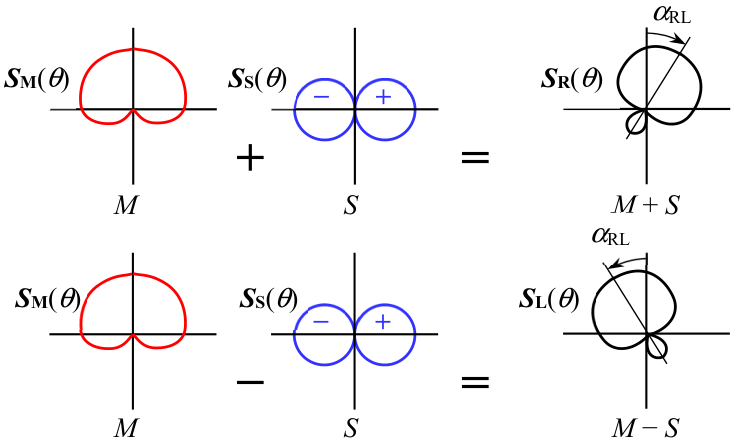
\includegraphics[width=0.8\linewidth]{Micros MS.png}
  Un micro cardioide y otro bidireccional. El ángulo $\alpha $ (que en las figuras aparece como $\alpha _{RL}$) representa el ángulo del cardioide producido con respecto al eje del conjunto de micrófonos.
  \begin{align*}
    S_R (\theta )               & = S_M (\theta ) + S_S (\theta )                                                \\
    S_L (\theta )               & = S_M (\theta ) - S_S (\theta )                                                \\
    S_0                         & = S_{M0} \left( A_M + \frac{B_M}{\cos (\alpha )} \right)                       \\
    \tan \left( \alpha  \right) & = \frac{S_{S0}}{B_M S_{M0}}                                                    \\
    B                           & = \frac{B_M}{A_M \cos (\alpha ) + B_M}                                         \\
    S_{M0}                      & = 2 S_0 \left[A_M + B_M \cos (\alpha ) \right]                                 \\
    S_{S0}                      & = 2 S_0 B_M \sin (\alpha )                                                     \\
    S_M ( \theta )              & = S_R ( \theta ) + S_L ( \theta ) = S_{M0} \left[ A + B \cos (\theta ) \right] \\
    S_S ( \theta )              & = S_R ( \theta ) - S_L ( \theta ) = S_{S0} \sen (\theta )
  \end{align*}

  \subsubsection{Técnica XY}
  Micros coincidentes, con ángulo de separación $\alpha$.
  \begin{align*}
    S_R (\theta )  & = S(\theta - \alpha )             \\
    S_L (\theta )  & = S(\theta + \alpha  )            \\
    S_M ( \theta ) & = S_R ( \theta ) + S_L ( \theta ) \\
    S_S ( \theta ) & = S_R ( \theta ) - S_L ( \theta )
  \end{align*}


  \subsection{Conexión eléctrica de los micrófonos}
  \subsubsection{Efecto del cable en la banda de frecuencias transmitida}
  Debido a capacidad entre hilos activos del cable, se produce un filtrado paso bajo. Cuanto más alta es la capacidad $C$ entre hilos activos del cable, más baja es la frecuencia de corte $\omega _H$ y más atenuación de agudos se produce. En micrófonos electrostáticos, si el cable se ubica entre la cápsula y el preamplicador se produce una atenuación muy severa en la banda de paso debida a la longitud del cable. Por este motivo, el preamplificador se sitúa junto a la cápsula y se le entrega alimentación ya sea a través de una pila o de una fuente de alimentación externa (Phantom, ICP, etc.).

  \subsubsection{Alimentación de micrófonos electrostáticos}

  La \textbf{alimentación Phantom} otorga una tensión continua al conjunto de cápsula electrostática y preamplificador. Es la más usada a nivel profesional. Suele ser de \qty{48}{\volt } pero puede trabajar bien entre \qty{12}{\volt } y \qty{52}{\volt } aproximadamente. Se entrega a través del propio cable de tres hilos y en modo común. Puede aportarse a los micrófonos dinámicos de bobina móvil sin que estos resulten dañados.

  La \textbf{alimentación CCP/IEPE/ICP} otorga una corriente continua y es usada principalmente en micrófonos electret de medición y acelerómetros. Utiliza conectores BNC.

  \newpage
  \section{T4. Sistemas de Refuerzo Sonoro}

  \subsection{Niveles acústicos}
  \subsubsection{Niveles de presión directa y reverberante con una única fuente}
  \begin{align*}
    p_d          & \equiv \text{Presión directa producida por el altavoz}                                                                                          \\\
    p_d          & = \left\lbrace
    \begin{matrix*}[l]
      \text{SPL}_d = L_W + 10 \log \left( \frac{Q(\theta, \varphi)}{4\pi r^2} \right)\\
      \text{SPL}_d = S + 10 \log \left( P_e \right) -20 \log \left( r \right) + D(\theta, \varphi) [\unit{\dB}]
    \end{matrix*} \right.                                          \\
    p_r          & \equiv \text{Presión reverberante producida por el altavoz (acústica estadística)}                                                              \\
    p_r          & = \left\lbrace
    \begin{matrix*}[l]
      \text{SPL}_r = L_W + 10 \log \left( \frac{4}{R} \right) \\
      \text{SPL}_r = 10 \log \left( P_a \right) - 10 \log \left( R \right) + 126 [\unit{\dB}] \\
      \text{SPL}_r = S + 10 \log \left( P_e \right) - 10 \log \left( Q _{\textnormal{ax}}R \right) + 17 [\unit{\dB}]
    \end{matrix*} \right.       \\
    p_t          & \equiv \text{Presión acústica total en el punto }P                                                                                              \\
    p_t          & = \sqrt{p_d^2 + p_r^2} = \sqrt{P_a \rho _0 c \left( \frac{Q(\theta, \varphi)}{4\pi r^2} + \frac{4}{R} \right)} \quad \text{(suma no coherente)} \\
    \text{SPL}_t & = L_W + 10 \log \left( \frac{Q(\theta, \varphi)}{4\pi r^2} + \frac{4}{R} \right) \quad \text{(ecuación de Hopkins-Stryker)}
  \end{align*}

  En EASE:
  \begin{itemize}
    \item $\text{SPL}_d$ se obtiene según geometría y electroacústica.
    \item $\text{SPL}_r$ (en realidad $\text{SPL}_t$) se obtiene mediante:
          \begin{itemize}
            \item Acústica estadística (\textbf{Standard Mapping}).
            \item Trazado de rayos, ya sea con \textbf{Standard With Reflections} (en desuso) o con \textbf{AURA}.
          \end{itemize}
  \end{itemize}
  \subsubsection{Constante acústica de la sala}
  La constante acústica de la sala $R$ representa la absorción total de sonido que producen las paredes del recinto. Depende de la frecuencia.
  \begin{align*}
     &  & \hat{\alpha} & = \frac{1}{S} \sum_{i}\alpha _i S_i       &  & = \underbrace{\frac{0.161V}{T_{60}S}} _{\text{Sabine}}                      &  & = \underbrace{1 - e ^{-\frac{0.161V}{T_{60}S}}} _{\text{Eyring}}                      \\
     &  & R            & = \frac{S \hat{\alpha}}{1 - \hat{\alpha}} &  & = \underbrace{\frac{S}{\frac{T_{60}S}{0.161 V} - 1}} _{\textnormal{Sabine}} &  & = \underbrace{S \left( e^{\frac{0.161V}{T_{60}S}} - 1 \right)} _{\textnormal{Eyring}}
  \end{align*}
  \subsubsection{Modificadores acústicos}

  \[ M_a = \frac{\left( 1 - \hat{\alpha} \right)Q _{\textnormal{ax}}}{\left( 1 - \alpha _1 \right)
    Q _{\textnormal{ideal}}} >1\]
  Standard Mapping no considera modificadores acústicos.

  \subsubsection{Distancia crítica}

  La distancia crítica $D_c$ es la distancia entre la fuente y los puntos a partir de los cuales la presión directa es igual a la presión reverberante.

  \[ D_c (\theta, \varphi) = 0.141 \sqrt{Q(\theta,\varphi)R} = \underbrace{0.141 \sqrt{Q _{\textnormal{ax}}R}} _{D_c(\ang{0},\ang{0})} D(\theta, \varphi) \]

  \begin{align*}
    D/R & \equiv \text{Relación de campo directo a campo reverberante} \\
    D/R & = \text{SPL}_d - \text{SPL}_r                                \\
  \end{align*}

  \subsubsection{Campo semirreverberante}
  \subsubsection{Niveles debidos a un número $M$ de fuentes}
  \begin{align*}
    \text{SPL}_{i}           & \equiv \text{Nivel que aporta la fuente }i                                                                                                                                         \\
    P _{a}                   & \equiv \text{Potencia acústica de la fuente}                                                                                                                                       \\
    P _{a \textnormal{ ref}} & \equiv \text{Potencia acústica de referencia} = \qty{1e-12}{\watt}                                                                                                                 \\
    \text{SPL}_{tc}          & = 20 \log \left( \sum_{i=1}^{M} 10^{\frac{\text{SPL}_i}{20}} \right)                                                                                                               \\
    \text{SPL}_{dt}          & = 10 \log \left( \sum_{i=1}^{M} 10^{\frac{\text{SPL}_{di}}{10}} \right) = 10 \log \left( \sum_{i=1}^{M} \frac{P_{ai}}{P_{a \textnormal{ ref}}} \cdot \frac{Q_i}{4\pi r_i^2}\right) \\
    \text{SPL}_{rt}          & = 10 \log \left( \sum_{i=1}^{M} 10^{\frac{\text{SPL}_{ri}}{10}} \right) = 10 \log \left( \sum_{i=1}^{M} \frac{P_{ai}}{P_{a \textnormal{ ref}}} \cdot \frac{4}{R}\right)            \\
    \text{SPL}_{tnc}         & = 10 \log \left( \sum_{i=1}^{M} 10^{\frac{\text{SPL}_i}{10}} \right)                                                                                                               \\
  \end{align*}
  El subíndice $c$ significa ``coherente'', mientras que $nc$ significa ``no coherente''. Además $d, r, t$ significan ``directo'', ``reverberante'' y ``total'' respectivamente.
  \subsubsection{Potencia acústica}

  \begin{align*}
    \text{Potencia acústica}           & \equiv P_a = \eta P_e                                                                                                                        \\
    \text{Potencia eléctrica aplicada} & \equiv P_e = \frac{E^2_{e}}{R_e} \ \text{o bien} \  \underbrace{P_e = \frac{E^2_e}{Z _{\textnormal{nom}}}}_{P \text{ entregada por el amp.}} \\
    \text{Eficiencia del altavoz}      & \equiv \eta = \left\lbrace
    \begin{matrix*}[l]
      10^{\frac{S - 10 \log \left( Q _{\textnormal{ax}} \right) -109 }{10}} & \text{si radiación en }4\pi s \\
      10^{\frac{S - 10 \log \left( Q _{\textnormal{ax}} \right) -112 }{10}} & \text{si radiación en }2\pi s \\
    \end{matrix*} \right.                                                                                                                      \\
  \end{align*}

  Hay que tener en cuenta las frecuencias de la señal y de medida cuando suministramos potencia eléctrica al altavoz. Si nos piden el $\text{SPL}_d$ generado por el altavoz en un punto en la banda de octava de \qty{1}{\kilo \hertz } y alimentamos al altavoz con un ruido de $N_B$ bandas de octava, entonces:

  \[ P_e \left( \text{octava de } \qty{1}{\kilo \hertz } \right) = \frac{P_{e} \left( \text{total} \right)}{N_B} \]

  Por lo tanto, si tenemos altavoces de tipo $\alpha, \beta$ que emiten una señal de $N_B$ octavas, la potencia se reparte entre todos de modo que:
  \[ P_{at} = \frac{M_{\alpha}\eta_{\alpha}P_{e\alpha \text{ máx}} + M_{\beta}\eta_{\beta}P_{e\beta \text{ máx}} }{N_B} \]

  Si hubiera más tipos de altavoces, se incluirían como los otros en el numerador de la fórmula anterior.


  \subsection{Respuesta temporal}
  \subsubsection{Molestia por ecos}
  \subsubsection{Efecto precedencia}
  \subsubsection{Respuesta temporal mediante simulación}
  \subsubsection{Auralización}

  \subsection{Inteligibilidad}
  \subsubsection{Índice de inteligibilidad del habla - SII}
  El índice de inteligibilidad del habla $I_{\textnormal{SII}}$ (\textit{Speech Intelligibility Index}) evalúa la SNR en la zona de audiencia para diferentes bandas de frecuencia.

  \begin{align*}
    \text{SII} & = \sum_{i=1}^{N_B}I_i A_i                              \\
    I_i        & \equiv \text{Coeficiente de importancia de la banda }i \\
    A_i        & \equiv \text{Audibilidad de la banda }i                \\
    N_B        & \equiv \text{Número de bandas usadas para el cálculo}  \\
  \end{align*}

  \subsubsection{Pérdida de articulación de consonantes - Alcons\%}
  Corresponde con el porcentaje de consonantes no entendidas con respecto a las consonantes emitidas.
  \[ \text{Alcons}\% = \frac{\text{Nº de consonantes no entendidas}}{\text{Nº de consonantes emitidas}} \times 100 \]

  Un valor de $0\%$ indica un resultado excelente pues se he entendieron todas las consonantes emitidas. Por otra parte, un valor de $100\%$ es un resultado pésimo que indica que no se entendió ninguna consonante.

  Si hay problemas usando ábaco:
  \begin{align*}
    R/N  & \equiv \text{Relación de campo reverberante a ruido}                                                \\
    R/N  & = \text{SPL}_r - \text{SPL}_N                                                                       \\
    D/RN & \equiv \text{Relación de campo directo a campo reverberante más ruido}                              \\
    D/RN & = \text{SPL}_d - 10 \log \left( 10^{\frac{\text{SPL}_r}{10}} + 10^{\frac{\text{SPL}_N}{10}} \right) \\
  \end{align*}
  \subsubsection{Índice de transmisión del habla - STI}

  El STI (\textit{Speech Transmission Index}) evalúa la pérdida de modulación de la intensidad acústica. Para calcularlo se siguen los siguientes pasos:
  \begin{enumerate}
    \item Se convierten los 98 índices de modulación $m$ en unidades logarítmicas (SNR aparente).
    \item Estos valores son truncados en el intervalo $\left[ \qty{-15}{\dB} , \qty{+15}{\dB}  \right]$.
    \item Se mapean los valores al intervalo $\left[ 0, 1 \right]$.
    \item Se promedian linealmente para las 14 frecuencia de modulación, obteniendo así 7 valores.
    \item Se promedian estos valores según unos coeficientes específicos para cada frecuencia y también en función de si se trata de una voz masculina o femenina.
  \end{enumerate}

  Entre los métodos habituales de medición del STI se encuentran:
  \begin{itemize}
    \item Se emite (a veces mediante altavoces que emulan el habla humana) una señal de banda ancha con modulaciones aplicadas y mediante procesado digital se calcula la intermodulación para cada valor de $m$.
    \item Se extraen los valores de $m$ a partir de la respuesta al impulso de la sala.
  \end{itemize}

  \subsection{Configuraciones de altavoces}
  \subsubsection{Sistema centralizado con un altavoz o un cluster}
  Una \textbf{isobara} $r_{\textnormal{SPL}}$ es el lugar geométrico de todos los puntos que tienen el mismo SPL.
  \begin{align*}
    \text{SPL}(r, \theta, \varphi)        & = S + 10 \log \left( P_e \right) - 20 \log r(\theta, \varphi)) + D_{\left( \unit{\dB} \right)}(\theta, \varphi)                                                                   \\
    r_{\textnormal{SPL}}(\theta, \varphi) & = 10^{ \frac{S + 10 \log \left( P_e \right) - \text{SPL}}{20} } \cdot 10 ^{\frac{D_{\unit{\dB}}(\theta, \varphi)}{20}} = r_{\textnormal{SPL}}(\ang{0},\ang{0}) D(\theta, \varphi)
  \end{align*}

  Si nos piden la cobertura a \qty{-6}{\dB} (o a los que sean) a partir de la directividad, evaluamos la directividad:
  \[ \theta _{L \left( \qty{-6}{\dB} \right)} = \alpha \quad \Longleftrightarrow \quad D \left( \frac{\alpha}{2} \right) = \qty{-6}{\dB}\]
  El \textbf{ángulo aparente de cobertura horizontal} $\theta ' _{\textnormal{LH}\left( \qty{-6}{\dB}  \right)}$ es la proyección sobre el suelo del ángulo de cobertura horizontal.

  \[ \theta ' _{\textnormal{LH}\left( \qty{-6}{\dB}  \right)} = 2 \arctan \left( \frac{\tan \left( \frac{\theta _{\textnormal{LH}\left( \qty{-6}{\dB}  \right)}}{2} \right)}{\cos (\phi)} \right) \]

  \subsubsection{Clusters y arrays de altavoces}

  Los \textbf{arrays circulares} consiguen aumentar la cobertura (reducir directividad). Suelen usarse en alta frecuencia.



  Los \textbf{arrays lineales} buscan reducir la cobertura (aumentar la directividad). Los ejes de los altavoces son paralelos para lograr suma coherente. Son apropiados para baja frecuencia.

  El término $b$ es la separación entre altavoces. Si el término $\frac{b}{\lambda}$ es grande, entonces se produce aliasing espacial y se produce mucho lobulado en la directividad del array. Si por el contrario $\frac{b}{\lambda}$ es pequeño, la directividad del array es prácticamente omnidireccional.

  El término $M$ es el número de altavoces del array. Si $M$ es grande, los lóbulos se hacen más directivos y habrá un mayor número de lóbulos secundarios.

  Los \textbf{arrays mixtos} son una combinación de los dos anteriores.

  Siendo $M$ el número de altavoces, entonces:
  \begin{align*}
    S \left( \text{array circular} \right) & = S \left( \text{altavoz} \right) - 10 \log \left( M \right) + K \\
    S \left( \text{array lineal} \right)   & = S \left( \text{altavoz} \right) + 10 \log \left( M \right)     \\
  \end{align*}

  \subsubsection{Sistema distribuidos de altavoces}
  \subsection{Realimentación acústica}

  La realimentación acústica es un fenómeno que se da cuando la señal acústica es captada, amplificada y emitida repetidamente en múltiples ciclos, generando efectos indeseados en la señal, como pueden ser:
  \begin{itemize}
    \item \textbf{Acople / oscilación / Efecto Larsen.} Se generan tonos puros de muy alto nivel que pueden dañar los equipos.
    \item \textbf{Coloración del espectro.}
    \item \textbf{Alargamiento de la respuesta temporal.}
  \end{itemize}

  \subsubsection{Modelo}
  \begin{center}
    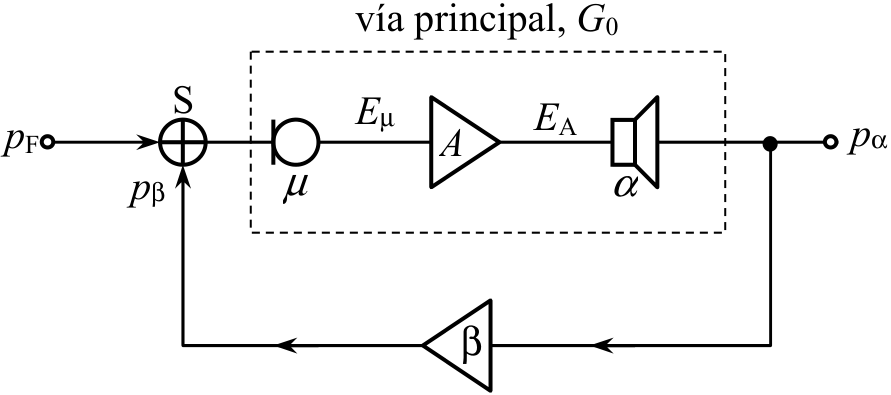
\includegraphics[width=0.7\linewidth]{Acople.png}
  \end{center}

  \begin{align*}
    \text{Ganancia de realimentación} \equiv G_R & = \frac{G_0}{1 - T}  \\
    \text{Ganancia de lazo} \equiv T             & = \mu A \alpha \beta \\
  \end{align*}

  Existen dos condiciones posibles para que se cumpla oscilación:
  \[ \left\lbrace
    \begin{matrix*}[l]
      \abs{T} = 1 & \text{Condición de nivel} \\
      \angle (T) = 2\pi n \quad n = 0,1,2, \ldots & \text{Condición de fase} \\
    \end{matrix*} \right. \]

  \subsubsection{Realimentación por un solo camino y en campo libre}
  Sucede cuando la señal acústica emitida por el altavoz llega directamente al micrófono.
  \subsubsection{Realimentación cuando existe reverberación}
  \subsubsection{Condición de oscilación según los niveles acústicos en los micrófonos}
  La condición de oscilación (incluyendo un margen de seguridad de \qty{6}{\dB} ) es:
  \[ \abs{T} = 0.5 \qquad \text{o en decibelios } \ \abs{T} = \qty{6}{\dB} \]
  Esta condición implica:
  \[ \text{SPL}_{Fd} = \text{SPL}_{\beta d} + D_{\mu \left( \unit{\dB} \right)} + \qty{6}{\dB} \]
  Donde:
  \begin{align*}
    \text{SPL}_{Fd}                   & \equiv \text{SPL}_d \text{ debido a la fuente}         \\
    \text{SPL}_{\beta d}              & \equiv \text{SPL}_d \text{ debido a la realimentación} \\
    D_{\mu \left( \unit{\dB} \right)} & \equiv \text{Directividad del micrófono}
  \end{align*}
  Se desprecia el efecto de la reverberación porque en la práctica esta expresión resulta más fácil de evaluar.

  \subsubsection{Respuesta temporal de la realimentación}
  \subsubsection{Control de la realimentación acústica}

  \subsection{Ganancia acústica}

  Para un orador (o fuente sin amplificar) en el punto $x$, tenemos:
  \begin{align*}
    \text{AG}                         & = \text{SPL}_{dx} - \text{SPL}_{\text{orador }x}                              \\
    \text{PAG}                        & = \text{SPL}_{dx \text{ potencial}} - \text{SPL}_{\text{orador }x}            \\
    \text{SPL}_{dx \text{ potencial}} & = \text{SPL}_{dx} - \qty{6}{\dB} \quad \text{(margen para evitar oscilación)} \\
  \end{align*}

  Se define la ganancia acústica \textbf{AG} (\textit{Acoustic Gain}) como el incremento de nivel que produce el sistema de refuerzo sonoro sobre la zona de audiencia con respecto al sistema apagado. La máxima ganancia acústica posible se ve limitada por el margen de \qty{6}{\dB} antes de que se produzca oscilación (acople). La mínima ganancia es determinada por el ruido de fondo de la sala.
  \subsubsection{Distancia acústica equivalente}
  La distancia acústica equivalente \textbf{EAD} (\textit{Equivalent Acoustic Distance}) es la distancia a la que el oyente sitúa subjetivamente al orador.
  \subsubsection{Ganancia acústica necesaria y ganancia acústica potencial}

  La ganancia acústica necesaria \textbf{NAG} (\textit{Needed Acoustic Gain}) es la ganancia acústica que garantiza que haya un $\text{SNR} > \qty{25}{\dB} $.

  La ganancia acústica potencial \textbf{PAG} (\textit{Potential Acoustic Gain}) es la ganancia acústica máxima que se puede conseguir sin que se produzca oscilación.

  \subsubsection{Uso de la ganancia acústica para el diseño de un sistema de refuerzo sonoro}

  Para evaluar un sistema de refuerzo sonoro usando la ganancia acústica:
  \begin{enumerate}
    \item Se busca la zona de audiencia más desfavorable.
    \item En dicho punto se calculan la NAG y la PAG.
    \item Si $\text{NAG} > \text{PAG}$, no se pueden cumplir los criterios de nivel y se tiene que rediseñar el sistema de refuerzo sonoro. Por lo general la NAG no puede disminuir, por lo que se busca aumentar la PAG.
    \item Si $\text{NAG} < \text{PAG}$, se busca una ganancia acústica cercana a la PAG.
  \end{enumerate}

  \subsection{Amplificación}

  El subíndice $\ell$ viene de ``línea''.
  \[ P_{e\ell} = E_{\ell} I_{\ell} = I_{\ell}^2 Z _{\textnormal{nom}} = \frac{E_{\ell}^2}{Z _{\textnormal{nom}}}\]

  \subsubsection{Amplificación de baja impedancia}
  En amplificación de baja impedancia, si se asegura que la carga de los altavoces es $Z _{\textnormal{nom}}$ entonces la potencia que manda es la que otorga el amplificador. Es decir, se busca la potencia máxima que admita la configuración de altavoces y se escoge un modo de amplificación que proporcione menos que esa.
  \subsubsection{Amplificación de alta impedancia, líneas de tensión constante}
  En amplificación de alta impedancia, si se asegura que la tensión de los altavoces es $E_{\ell}$ entonces la potencia que manda es la que se disipa en los altavoces. Es decir, se busca la configuración de altavoces que proporcione $E_{\ell}$ a la salida y se escoge un modo de amplificación que proporcione esa tensión y no supere la potencia máxima del amplificador.
  \subsubsection{Conexión de amplificadores}
  \begin{center}
    \textbf{Modo puente o \textit{bridge}}

    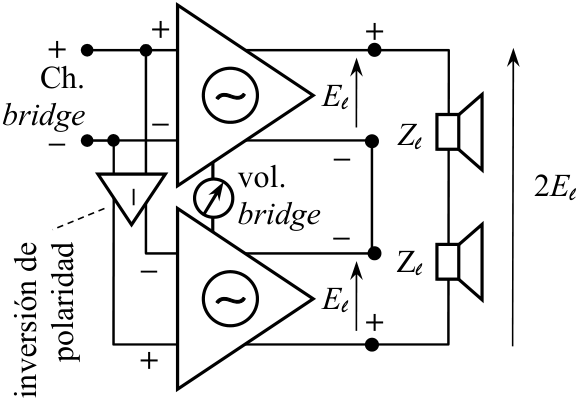
\includegraphics[width=0.5\linewidth]{Amp-bridge.png}

    \vspace{5pt}
    \textbf{Modo paralelo}

    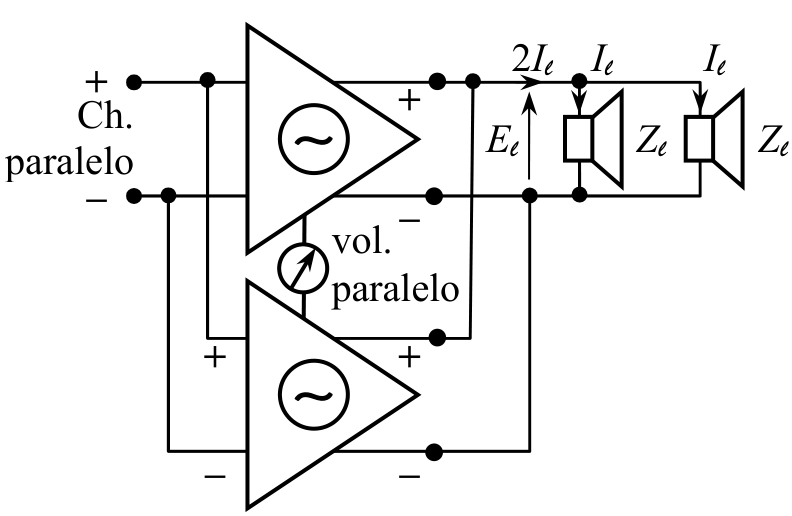
\includegraphics[width=0.5\linewidth]{Amp-paralelo.png}
  \end{center}
  \subsubsection{Clases de amplificación}
  \subsubsection{Fuentes de alimentación}

\end{multicols}

\end{document}
